\section{String Diagram Rewrite Theory}\label{sec:combinatorial-semantics}

In this section,  we recall the fundamental definitions and results of string diagram rewrite theory for symmetric monoidal categories,  building to the recapitulation of the correspondence between string diagram rewriting and an appropriate notion of double pushout (DPO) rewriting of certain hypergraphs,  as established in~\cite{bonchi_string_2022-1, bonchi_string_2022-2}.  

First,  we fix some notation.  Let $(-)^*$ be the free monoid monad over \textsf{Set}.  
We extend this to the case of relations $R \subseteq V \times V$,  so that we denote by $R^{*} \subseteq V^* \times V^*$ the element-wise extension of $R$ to a relation on ordered sequences. 
We will sometimes use functional notation for relations,  so that given $R \subseteq V \times W$ and $v \in V$,  $R(v) \subseteq W$. 
We elide associativity and unit isomorphisms associated with coproducts $(+)$,  and denote by $\iota_j: X_{j} \rightarrow X_{1} + \ldots X_{j} + \ldots X_{n}$ the $j^{\text{th}}$ injection,  and $[f,g]: A_1 + A_2 \to B$ the co-pairing of two morphisms $f: A_1 \to B$ and $g:A_2 \to B$. 
We denote by $A +_{f,g} B$ the pushout of the span $A \xleftarrow{f} C \xrightarrow{g} B$.
We will also refer to $A,B$ as \textit{feet} of the cospan, and to $C$ as \textit{carrier}.

\subsection{Hypergraphs}

In ~\cite{bonchi_string_2022-1},  hypergraphs \textit{with interfaces} and their DPO rewriting are shown to be sound and complete for categorical presentations of SMTs including a Frobenius algebra. 
Hypergraphs generalise graphs by allowing edges to have multiple sources and targets. 
When interpreting string diagrams as hypergraphs,  morphisms are interpreted as edges,  and wires as vertices.  
However,  there is also a need to specify which vertices are to be considered as \textit{input} and \textit{outputs},  corresponding to the dangling wires at the bottom and top of a string diagram. 
This gives rise to the definition of a hypergraph with interfaces.  
Subsequent work \cite{bonchi_string_2022-2} builds on this correspondence to give a restriction of hypergraphs with interfaces (called \textit{monogamous} directed acyclic),  leading to a correspondence between symmetric monoidal string diagrams (\textit{i.e.}, without requiring a Frobenius algebra) and the category of such hypergraphs.


\begin{definition}[Category of hypergraphs]\label{def:hypergraph}
A \emph{hypergraph $\mathcal{G}$ over a signature $\Sigma$} is a tuple $(V,E,s,t,l)$,  where $V$ is a finite set of vertices, $E$ is a finite set of edges, $s : E \to V^{*}$ is a source function, $t : E \to V^{*}$ is a target function,  and $l : E \to \Sigma$ is a labelling function that assigns each edge a generator from monoidal signature $\Sigma$.  The labelling function must respect the typing of the generator: for all edges $e$,  $|s(e)| = m$ and $|t(e)| = n$,  where $l(e) : m \to n$.  We call a hypergraph \textit{discrete} if its set of edges is empty.   
A \emph{hypergraph homomorphism} $\phi: \mathcal{F} \to \mathcal{G}$ is given by a pair of functions $\phi_V : V_{\mathcal{F}} \to V_{\mathcal{G}}, \phi_E : E_{\mathcal{F}} \to E_{\mathcal{G}}$ such that the following hold. 
\begin{enumerate}
    \item $\phi_V^*(s_{\mathcal{F}}(e)) = s_{\mathcal{G}}(\phi_E(e))$
    \item $\phi_V^*(t_{\mathcal{F}}(e)) = t_{\mathcal{G}}(\phi_E(e))$
    \item $l_{\mathcal{F}}(e) = l_{\mathcal{G}}(\phi_E(e))$
\end{enumerate}
We denote by $\catname{Hyp(\Sigma)}$ the category of hypergraphs over $\Sigma$ and hypergraph homomorphisms. 
\end{definition}
Note that $\catname{Hyp(\Sigma)}$ has all finite colimits and, in particular,  the coproduct is given by the disjoint union of hypergraphs.
The initial object is given by the empty hypergraph.  

\begin{definition}[Symmetric monoidal category of cospans]
Let $\mathbb{C}$ be a category with all finite colimits.  A cospan from $X$ to $Y$ is a pair of arrows $X \xrightarrow{} A \xleftarrow{} Y$  in $\mathbb{C}$.  This \textit{category of cospans of $\mathbb{C}$},  denoted $\catname{Csp(\mathbb{C})}$,  has as objects those of $\mathbb{C}$ and as arrows isomorphism classes of cospans.
%Two cospans $X \xrightarrow{} A \xleftarrow{} Y$ and $X \xrightarrow{} B \xleftarrow{} Y$ are isomorphic if the following diagram commutes and $\alpha$ is iso.
%\[
%\begin{tikzcd}
%                                               & A \arrow[dd, "\alpha"] &                                                \\
%X \arrow[ru, bend left] \arrow[rd, bend right] &                        & Y \arrow[ld, bend left] \arrow[lu, bend right] \\
%                                               & B                      &                                               
%\end{tikzcd}
%\]
%For $X \in \mathbb{C}$ an $id$-cospan is $X \xrightarrow{id_X} X \xleftarrow{id_X} X$.
Composition of cospans $X \xrightarrow{f} A \xleftarrow{g} Y$ and $Y \xrightarrow{h} B \xleftarrow{i} Z$ is given by pushout: $X \xrightarrow{f} A +_{g,h} B \xleftarrow{i} Z$,  with identity given by the cospan of identities.  Its monoidal product is given by the coproduct of $\mathbb{C}$ as follows: 
\ifdefined \ONECOLUMN
\[
    (A \xrightarrow{f} \mathcal{G} \xleftarrow{g} B) \otimes (A' \xrightarrow{f'} \mathcal{G'} \xleftarrow{g'} B') \coloneq A + A' \xrightarrow{f+f'} \mathcal{G} + \mathcal{G'} \xleftarrow{g+g'} B + B'  ,
\]
\else
\begin{multline*}
    (A \xrightarrow{f} \mathcal{G} \xleftarrow{g} B) \otimes (A' \xrightarrow{f'} \mathcal{G'} \xleftarrow{g'} B') \coloneq\\ A + A' \xrightarrow{f+f'} \mathcal{G} + \mathcal{G'} \xleftarrow{g+g'} B + B'  , 
\end{multline*}
\fi
and its unit by the initial object of $\mathbb{C}$.
Symmetry is inherited from $\mathbb{C}$ as the coproduct~\cite{MonoidalCoproduct}.
\end{definition}


Then, morphisms of $\catname{S}(\Sigma)$ can be interpreted as particular cospans of discrete hypergraphs,  which we call hypergraphs with interfaces~\cite{bonchi_string_2022-2}.
\begin{definition}[Hypergraphs with interfaces]
\label{def:cspd}
Define the category of \emph{hypergraphs with interfaces} $\catname{HypI(\Sigma)}$ as the full sub-category of $\catname{Csp(Hyp(\Sigma))}$ with discrete hypergraphs as objects.
\end{definition}

In particular, this means that any morphism in $\HypI{\Sigma}$ is of the form $n \xrightarrow{f} \mathcal{G} \xleftarrow{g} m$,
where $n,\;m$ are discrete hypergraphs and $\mathcal{G}$ is an arbitrary hypergraph.  The morphisms $f$ and $g$ into $\mathcal{G}$ will specify which vertices are to be considered as inputs and outputs,  respectively.   

\begin{definition}[Degree,  path,  acyclic] 
The \emph{in-degree} of a vertex $v$ in a hypergraph $\mathcal{G}$ is the number of hyperedges $e \in {E_\mathcal{G}}$ such that $v \in t(e)$.  
Similarly, the out-degree of $v$ is the number of edges $e \in E_\mathcal{G}$ such that $v \in s(e)$.
A \emph{path} from $e_0$ to $e_{n-1}$ of length $n$ in a hypergraph $\mathcal{G}$ is an ordered sequence of edges $[e_0, e_1, \ldots, e_{n-1}] \in E_\mathcal{G}^*$ such that for all $i < n - 1$ some vertex $v \in t(e_i)$ is also in $s(e_{i+1})$.
A hypergraph is \emph{directed acyclic} if it contains no paths of length $n > 0$ that start and end in the same edge.
\end{definition}

In order to represent only morphisms of $\catname{S}(\Sigma)$,  it is necessary to restrict our attention to the following subset of hypergraphs with interfaces. 
\begin{definition}[Category of MDA Hypergraphs with Interfaces]
\label{def:monogamy_hyp}
We call a cospan $n \xrightarrow{f} \mathcal{G} \xleftarrow{g} m$ in $\HypI{\Sigma}$ \emph{monogamous directed acyclic (MDA)} if:
\begin{enumerate}
    \item $\mathcal{G}$ is a directed acyclic hypergraph;
    \item $f$ and $g$ are monomorphisms;
    \item the in-degree and out-degree of every vertex is at most $1$;
    \item vertices with in-degree $0$ are precisely the image of $f$; and
    \item vertices with out-degree $0$ are precisely the image of $g$.
\end{enumerate}
We denote by $\MdaCospans$ the subcategory of $\HypI{\Sigma}$ of MDA cospans.
\end{definition}
Note that $\MdaCospans$ remains a symmetric monoidal category with the same equipment as before.  We now recall from
\cite{bonchi_string_2022-2} the following theorem,  which says the category $\MdaCospans$ is in fact \textit{equivalent} to $\catname{S}(\Sigma)$. 
\begin{theorem}[Corollary 26 of~\cite{bonchi_string_2022-2}]\label{thm:prop-equiv}
    $\catname{S}(\Sigma) \cong \MdaCospans$
\end{theorem}

\subsection{DPOI-Rewriting for Hypergraphs with Interfaces}
The correspondence of the previous section means that the symmetric monoidal equations of $\catname{S}(\Sigma, \mathcal{E})$ are absorbed in the hypergraph representation.  The equations $\mathcal{E}$ are then to be considered as rewrite rules on string diagrams,  which are then modelled as DPO-rewrites on hypergraphs with interfaces. 
DPO rewriting is a standard technique for formalising graph rewriting categorically. 
In this section we recall standard results of double-pushout (DPO) rewriting of hypergraphs,  as well as the specific notion of DPO rewriting which is sound and complete for arbitrary SMTs,  which is called \textit{convex} rewriting. 

The intuitive notion of (hyper-)graph rewriting is  as expected: given a rewrite rule $\mathcal L \rightsquigarrow \mathcal R$ and a graph $\mathcal{G}$,  we expect to find an occurrence of $\mathcal L$ within $\mathcal{G}$,  remove it,  and then plug $\mathcal R$ into the hole to recover the rewritten graph $\mathcal{H}$.  In DPO rewriting,  such a rewrite rule is formalised as a span $\mathcal L \xleftarrow{} \mathcal K \xrightarrow{} \mathcal R$ in some appropriate category of graphs,  where $\mathcal K$ is some invariant that should be maintained during rewriting.
A typical DPO square is depicted in Figure~\ref{fig:dpo_dpoi}~(left).

% \[
% \begin{tikzcd}
% \mathcal L \arrow[d, "m"'] & \mathcal K \arrow[d] \arrow[l] \arrow[r] & \mathcal R \arrow[d]   \\
% \mathcal G^{\urcorner}     & \mathcal C \arrow[l] \arrow[r] & ^{\ulcorner} \mathcal H
% \end{tikzcd}
% \]
% CHRIS: WHY IS J DISPLAYING AND NOT R? 
% \[
%     \scalebox{0.8}{
%         \tikzfig{combinatorial_semantics/DPO_square}
%     }
% \]

The morphism $\mathcal L \to \mathcal G$ is called a \textit{match},  defined whenever there is a corresponding \textit{pushout complement}---the pair of morphisms $\mathcal K \to \mathcal \mathcal{L}^{\bot} \to \mathcal G$ completing the top half of the pushout square defined by $\mathcal K \xrightarrow{} \mathcal L \xrightarrow{} \mathcal G$. 
When the morphisms involved in the rewrite rule are monomorphisms,  as is usually required,  constructing $\mathcal{L}^{\bot}$ can be intuitively understood as finding an occurrence of $\mathcal L$ in $\mathcal G$ and removing from this occurrence everything that has no pre-image in $\mathcal K$.  The final graph $\mathcal H$ is then recovered by inserting into the hole everything from $\mathcal R$ that has no pre-image in $\mathcal K$ --- hence the two pushouts: one for deletion and one for insertion.  In this case,  we say that $\mathcal G$ is rewritten into $\mathcal H$ via the rewrite rule $\mathcal L \xleftarrow{} \mathcal K \xrightarrow{} \mathcal R$.

To express the rewriting of (hyper-)graphs with interfaces,  \textit{i.e.},  the ones that represent morphisms in $\HypI{\Sigma}$, the DPO formalism has been extended to double-pushout rewriting with \textit{interfaces}  (DPOI) as shown in Figure~\ref{fig:dpo_dpoi}~(right).
In the case of $ \catname{Hyp(\Sigma)}$,  we wish rewrite rules to be pairs of discrete cospans of hypergraphs with matching interfaces: $n \xrightarrow{} \mathcal L \xleftarrow{} m$, $n \xrightarrow{} \mathcal R \xleftarrow{} m$.  
By noting that a cospan $0 \xrightarrow{} \mathcal L \xleftarrow{[f,g]} n + m$ encodes the same data as a cospan $n \xrightarrow{f} \mathcal L \xleftarrow{g} m$ (Remark 3.14~\cite{bonchi_string_2022-1}) we can formulate a rewrite rule as a single span $\mathcal L \xleftarrow{} n+m \xrightarrow{} \mathcal R$,  and we can do similarly for the discrete cospans giving the interface to $\mathcal G$ and $\mathcal H$.  
We now make this identification throughout without further mention.  
Thus we reach the following variant of DPO rewriting.
\begin{definition}[DPOI rewriting]\label{def:dpoi}
Given a span of morphisms $\mathcal G \xleftarrow{} n+m \xrightarrow{} \mathcal H$ in $\textbf{Hyp}(\Sigma)$,  we say \textit{$\mathcal G$ rewrites to $\mathcal H$ with interface $n+m$ via rewrite rule $\mathcal L \xleftarrow{} i+j \xrightarrow{} \mathcal R$} if there exists an object $\mathcal C$ and morphisms which complete the rightmost commutative diagram in Figure~\ref{fig:dpo_dpoi} such that the two marked squares are pushouts.
% \[
% \begin{tikzcd}
% \mathcal L \arrow[d, "m"'] & i+j \arrow[d] \arrow[l] \arrow[r] & \mathcal R \arrow[d]   \\
% \mathcal{G}^{\urcorner}     & \mathcal C \arrow[l] \arrow[r]                      & ^{\ulcorner}\mathcal H \\
%                   & n+m \arrow[lu] \arrow[u] \arrow[ru]          &              
% \end{tikzcd}
% \]
\begin{figure}[t!]
    \begin{subfigure}[T]{0.4\linewidth}
    \[
                % \tikzfig{../figures/combinatorial_semantics/DPO_square}
                \begin{tikzcd}
                    {\mathcal{L}} & {\mathcal{K}} & {\mathcal{R}} \\
                    {\mathcal{G}} & {\mathcal{L}^{\bot}} & {\mathcal{H}}
                    \arrow["f"', from=1-1, to=2-1]
                    \arrow[from=1-2, to=1-1]
                    \arrow[from=1-2, to=1-3]
                    \arrow[from=1-2, to=2-2]
                    \arrow[from=1-3, to=2-3]
                    \arrow["\lrcorner"{anchor=center, pos=0.125, rotate=90}, draw=none, from=2-1, to=1-2]
                    \arrow[from=2-2, to=2-1]
                    \arrow[from=2-2, to=2-3]
                    \arrow["\lrcorner"{anchor=center, pos=0.125, rotate=180}, draw=none, from=2-3, to=1-2]
                \end{tikzcd}
    \]
    % \subcaption{DPO square}
    % \label{fig:dpo}
    \end{subfigure}
    \hfill
    \begin{subfigure}[T]{0.4\linewidth}
        \[
    % \scalebox{0.8}{
        % \tikzfig{../figures/combinatorial_semantics/DPOI_square_Hyp}
    % }
    \begin{tikzcd}
        {\mathcal{L}} & {i+j} & {\mathcal{R}} \\
        {\mathcal{G}} & {\mathcal{L}^{\bot}} & {\mathcal{H}} \\
        & {n+m}
        \arrow["f"', from=1-1, to=2-1]
        \arrow[from=1-2, to=1-1]
        \arrow[from=1-2, to=1-3]
        \arrow[from=1-2, to=2-2]
        \arrow[from=1-3, to=2-3]
        \arrow["\lrcorner"{anchor=center, pos=0.125, rotate=90}, draw=none, from=2-1, to=1-2]
        \arrow[from=2-2, to=2-1]
        \arrow[from=2-2, to=2-3]
        \arrow["\lrcorner"{anchor=center, pos=0.125, rotate=180}, draw=none, from=2-3, to=1-2]
        \arrow[from=3-2, to=2-1]
        \arrow[from=3-2, to=2-2]
        \arrow[from=3-2, to=2-3]
    \end{tikzcd}
\]
    % \subcaption{DPOI square}
    % \label{fig:dpoi}
    \end{subfigure}
    \captionsetup{belowskip=-3ex}
    \caption{DPO and DPOI squares}
    \label{fig:dpo_dpoi}
\end{figure}

\end{definition}
We need to restrict the notions of pushout complement and of match in order to preserve monogamy and directed acyclicity.  

\begin{definition}[Boundary complement]
\label{def:boundary_original}
For MDA cospans $i \xrightarrow{a_1} L \xleftarrow{a_2} j$ and $n \xrightarrow{b_1} \mathcal G \xleftarrow{b_2} m$
and mono $f : \mathcal L \to \mathcal G$, a pushout complement $i + j \to \mathcal{L}^\bot \to \mathcal G$ as depicted in the square below
% \begin{figure}[h!]
%     \centering
%     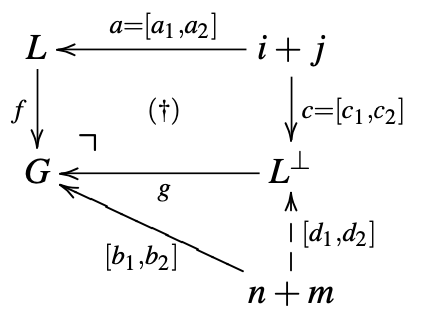
\includegraphics[width=0.4\linewidth]{figures/combinatorial_semantics/boundary_complement.png}
% \end{figure}
% https://q.uiver.app/#q=WzAsNSxbMCwwLCJMIl0sWzIsMCwiaStqIl0sWzAsMiwiR157XFx1cmNvcm5lcn0iXSxbMiw0LCJuK20iXSxbMiwyLCJMXntcXGJvdH0iXSxbMyw0LCJbZF8xLGRfMl0iLDJdLFszLDIsIltiXzEsYl8yXSJdLFswLDIsImYiLDJdLFsxLDAsImEgPSBbYV8xLGFfMl0iLDJdLFsxLDQsImMgPSBbY18xLGNfMl0iXSxbNCwyLCJnIl1d
% \[\begin{tikzcd}
% 	\mathcal L && {i+j} \\
% 	\\
% 	{\mathcal G^{\urcorner}} && {\mathcal{L}^{\bot}} \\
% 	\\
% 	&& {n+m}
% 	\arrow["{[d_1,d_2]}"', from=5-3, to=3-3]
% 	\arrow["{[b_1,b_2]}", from=5-3, to=3-1]
% 	\arrow["f"', from=1-1, to=3-1]
% 	\arrow["{[a_1,a_2]}"', from=1-3, to=1-1]
% 	\arrow["{[c_1,c_2]}", from=1-3, to=3-3]
% 	\arrow[from=3-3, to=3-1]
% \end{tikzcd}\]
\[
    \scalebox{0.8}{
        \tikzfig{../figures/combinatorial_semantics/DPOI_boundary_complement}
    }
\]
is called a boundary complement if $[c_1, c_2]$ is mono and there exist $d_1 : n \to \mathcal{L}^{\bot}$ and $d_2 : m \to \mathcal{L}^{\bot}$ making the above triangle commute and such that
\[
    n + j \xrightarrow{[d_1,c_2]} \mathcal{L}^{\bot} \xleftarrow{[d_2,c_1]} m + i
\]
is an MDA cospan. 
\end{definition}
%\begin{remark}
%    Note how the requirement for $i \xrightarrow{} L \xleftarrow{} j$ and $n \xrightarrow{} G \xleftarrow{} m$ being monogamous, i.e. morphisms in $\MdaCospans$, is a part of the above definition.
%\end{remark}
Intuitively,  requiring boundary complements ensures that inputs are glued exclusively to outputs and vice-versa in the two pushout squares.
Yet, this restriction is not enough to make DPOI rewriting complete for $\catname{S,\mathcal{E}}$: there might be cospans with carriers $\mathcal{G}$ and $\mathcal{H}$ such that one can be rewritten into another but their corresponding morphisms are not equal modulo $\mathcal{E}$~\cite{bonchi_string_2022-1}.
To make the DPOI rewriting complete, we need to add a restriction on the image of the match.

\begin{definition}[Convex match]
We call a subgraph $\mathcal{H}$ of a hypergraph $\mathcal{G}$ a \emph{convex subgraph} if for all $v_i, v_j \in V_{\mathcal{H}}$ every path from $v_i$ to $v_j$ is also in $\mathcal{H}$.
We call a match $f : \mathcal L \to \mathcal G$ a \emph{convex match} if it is mono and its image is a convex subgraph of $\mathcal G$. 
   
\end{definition}

\begin{definition}[Convex DPOI rewriting]
\label{def:convex_dpo}
Let $\mathfrak{R}$ be a set of DPOI rewrite rules. 
Then, given $\mathcal G \xleftarrow{} n+m$ and $\mathcal H \xleftarrow{} n + m$ in $\catname{Hyp(\Sigma)}$, $\mathcal G$ rewrites convexly into $\mathcal H$ with interface $n + m$ --- notation $(\mathcal G \xleftarrow{} n + m ) \Rrightarrow_{\mathfrak{R}}  (\mathcal H \xleftarrow{} n + m )$ --- if there exist rule $\mathcal L \xleftarrow{} i + j \xrightarrow{} \mathcal R$ in $\mathfrak{R}$ and object $\mathcal{L}^{\bot}$ and cospan arrows $i+j \xrightarrow{} \mathcal{L}^{\bot} \xleftarrow{} n+m$ such that the DPOI diagram of Definition \ref{def:dpoi} commutes and its marked squares are pushouts 
and the following conditions hold
\begin{itemize}
    \item $f : L \to \mathcal G$ is a convex match;
    \item $i + j \to \mathcal{L}^{\bot} \to \mathcal G$ is a boundary complement in the leftmost pushout.
\end{itemize}
\end{definition}
%By requiring convex matching and boundary complements we ensure that the original cospans above are monogamous, e.g., $n \xrightarrow{} G \xleftarrow{} m$.
We do not formally recite the main result of \cite{bonchi_string_2022-2} here,  but the work proves that for any morphisms $f$ and $g$ in $\catname{S}(\Sigma, \mathcal{E})$,  we have that $f = g$ if and only if there exist a sequence of DPO rewrites (induced by $\mathcal{E}$) between the representations of $f$ and $g$ as hypergraphs.  In particular,  Theorem \ref{thm:prop-equiv} means that the structural SMC equations are factored out in the representation of $f$ and $g$,  and the DPO rewrites necessary are only those induced by $\mathcal{E}$. 
%\begin{theorem}[Theorem 35~\cite{bonchi_string_2022-2}]
%For any $f,g \in \mathbf{SMT}(\Sigma, \mathcal{E})$,  we have that 
%\[
%	f = g \iff \llangle \lceil f \rceil \rrangle \Rrightarrow^*_{\mathfrak{R}} \llangle \lceil g \rceil \rrangle~, 
%\]
%where $\mathfrak{R} = \llangle \lceil \mathcal{E} \rceil \rrangle$ and $ \Rrightarrow^*_{\mathfrak{R}}$ denotes the existence of a sequence of convex rewrites. 
%\end{theorem}